\chapter{Estado de la cuestión}
\label{chap:antecedentes}

\drop{E}{}n este capítulo se lleva a cabo una prospección de los sistemas y artículos
que se han efectuado hasta la fecha, de modo que se contextualice el \acs{TFG} en el ámbito 
de la utilización de \acs{UAV}s, en diferentes ámbitos de la ingeniería civil en general y, más
concretamente, en situaciones de emergencia. Asimismo se analizarán las tecnologías de mayor 
relevancia para el desarrollo e implementación del sistema adaptativo.  

\section{Vehículo aéreo no tripulado}
\label{sec:vehiculonotripulado}

La aviación no tripulada comprende una amplia gama de aeronaves. El origen de estas aeronaves no tripuladas reside 
en la creación de los torpedos aéreos, que después evolucionaron a través de las bombas guiadas, los blancos 
aéreos (o drones), los señuelos, los modelos deportivos de radiocontrol, las aeronaves de investigación, 
las aeronaves de reconocimiento y las aeronaves de combate.

Un \acs{UAV} es «un  vehículo  aéreo  motorizado  que no  lleva  a  bordo  a  un  operador  humano,  
que utiliza las fuerzas aerodinámicas para proporcionar la elevación del vehículo, que puede volar autónomamente 
o ser tripulado por control remoto, que puede ser sustituido o recuperado, y que puede transportar una 
carga letal o no» \cite{UAV}. Dada esta definición quedan excluidos:

\begin{itemize}
\item Los planeadores, debido a que no usan una planta propulsora.
\item Los globos y dirigibles, ya que no se elevan mediante fuerzas aerodinámicas sino mediante fuerzas de flotabilidad.
\item Los misiles balísticos, misiles de crucero y proyectiles de artillería.
\end{itemize}

La palabra \acs{UAV} se comienza a hacer frecuente en los años 90 para representar a las aeronaves robóticas 
y así, reemplazar el término vehículo aéreo pilotado remotamente o \acs{RPV}. \acs{UAV} y \acs{RPV} no son más 
que dos nombres entre aproximadamente la docena que han recibido las aeronaves robóticas no tripuladas a lo largo de la historia (ver Figura~\ref{fig:cronologia}).

«En el año 2011 la Organización de Aviación Civil Internacional, organismo especializado de las Naciones 
Unidas para la aviación civil y del cual España forma parte al haber suscrito el Convenio de Chicago de 1944, 
publicó su Circular 328 en la cual por vez primera reconoce a las aeronaves no tripuladas como aeronaves, 
con todo lo que ello trae consigo, y de entre todas las posibles tipologías escoge a las que se pilotan de manera 
remota para ser consideradas como aptas para la aviación civil» \cite{dron1}.

\begin{figure}[!h]
\begin{center}
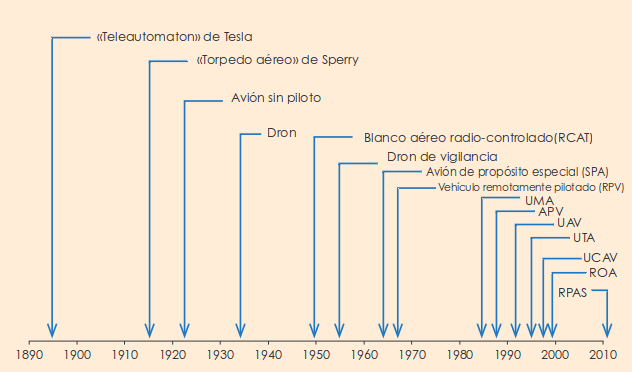
\includegraphics[width=0.8\textwidth]{/cronologia1.jpg}
\caption[Caption]{Cronología de los nombres aplicados a las aeronaves robóticas\footnotemark}
\label{fig:cronologia}
\end{center}
\end{figure}

\footnotetext{Los acrónimos no especificados se corresponden con: UMA = Unmanned Aircraft, 
APV = Automatically Piloted Vehicle, UTA = Unmanned Tactical Aircraft, UCAV = Unmanned Combat Air Vehicle, 
ROA = Remotely Operated Aircraft.}

\subsection{Historia}

Los europeos fueron pioneros en el desarrollo de los principios de la aeronáutica y, al 
tratar de emplearlos en aeronaves, volaron modelos no tripulados que pueden ser los primeros vehículos 
aéreos no tripulados de la historia. Precursores de la aviación en distintos países siguieron una progresión que va de los
planeadores a los aviones propulsados no tripulados, y de los vuelos no tripulados a los
tripulados (ver Cuadro~\ref{tab:pioneros}). Su limitación tecnológica, no disponer de un motor con suficiente relación potencia-peso, 
impidió que sus diseños pudieran mantenerse en el aire.

\begin{table}[hp]
  \centering
  {\small
  \begin{tabular}{p{.1\textwidth}p{.2\textwidth}p{.18\textwidth}p{.17\textwidth}p{.2\textwidth}}
  \tabheadformat
  \tabhead{País} &
  \tabhead{Planeador no tripulado} &
  \tabhead{Planeador tripulado} &
  \tabhead{Avión no tripulado}  &
  \tabhead{Avión tripulado}	\\
\hline
\textit{Inglaterra}  & Cayley, 1809 & Cayley, 1849 & Cody, 1907 & Cody, 1908 \\
                 
\hline
\textit{Francia} &  & Ferber, 1901 & Du Temple, 1857 & Santos-Dumont, 1906 \\
                       
\hline
\textit{Alemania}  &  & Lilienthal, 1891 &  &  \\
                       
\hline
\textit{Japón}  &  & Leprieur/Aibara, 1909 & Ninomiya, 1891 & Nagahara, 1911 \\
                      
\hline
\textit{Rusia}  &  &  &  & Rossinsky, 1910 \\
                   
\hline
\textit{Estados Unidos}  &  & Chanute, 1896 & Langley, 1896 & Hnos. Wright, 1903  \\
                      
\hline
\end{tabular}


% Local variables:
%   coding: utf-8
%   ispell-local-dictionary: "castellano8"
%   TeX-master: "main.tex"
% End:

  }
  \caption[Primeros vuelos conocidos en diversos países]
  {Primeros vuelos conocidos en diversos países \cite{dron1}}
  \label{tab:pioneros}
\end{table}

Durante la \textbf{Primera Guerra Mundial}, la aviación no tripulada se veía entorpecida por falta de desarrollo tecnológico. 
Los obstáculos se encontraban en los problemas de estabilización automática, control remoto y navegación autónoma. Fue Elmer Sperry el primero en resolver estos inconvenientes en una aeronave no tripulada. Elmer Sperry creó un giroestabilizador para un avión en \textbf{1909}, que tenía un rendimiento mediocre y era demasiado pesado. Ayudado por Glenn Hammond Curtiss optimizó su invento, que ahora era 
más pequeño y permitía controlar el avión en los tres ejes.

En \textbf{1916} se realiza la primera demostración del mecanismo de Sperry para guiar un avión convencional, 
el Hewitt-Sperry Automatic Airplane. Para efectuar la prueba, el aviador debía levantar el vuelo antes de activar el piloto automático. Después el avión volaba una ruta previamente programada y picaba. El piloto recuperaba el control de la aeronave en dicho momento y retornaba al aeródromo.

Finalmente, tras dos años de intentos fallidos, el torpedo aéreo de Sperry (ver Figura~\ref{fig:hewittsperry}) hizo un vuelo de 900 metros, el \textbf{6 de marzo de 1918}, siendo el primer viaje exitoso de un avión no tripulado en la historia. Su método de guiado para llegar al objetivo era primitivo pero ingenioso. Una vez que se conocía el viento y la distancia al objetivo, se calculaban las revoluciones necesarias para acertar en el blanco. Una vez alcanzadas las revoluciones precisas, se separaban las alas del fuselaje, dejando caer el torpedo sobre el objetivo.

\begin{figure}[!h]
\begin{center}
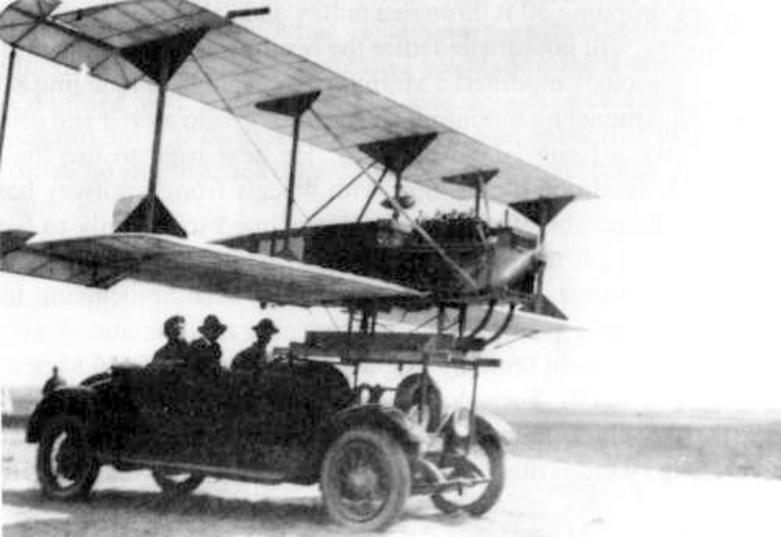
\includegraphics[width=0.8\textwidth]{/Hewitt-Sperry.jpg}
\caption[Caption]{Torpedo aéreo de Sperry}
\label{fig:hewittsperry}
\end{center}
\end{figure}

Los primeros sistemas se desarrollaron como armamento de largo alcance en artefactos tales como el torpedo aéreo de Sperry, mencionado anteriormente, y el blanco aéreo británico Aerial Target. El Aerial Target era un monoplano, sin piloto, controlado por radio que sirvió para verificar la viabilidad de utilizar señales de radio como sistema de guiado.

En el transcurso de la \textbf{Segunda Guerra Mundial}, Gran Bretaña abandonó la elaboración de misiles de crucero y se introdujo en el sector de los blancos aéreos con control completo por radio, a pesar de que el alcance era muy limitado.
En paralelo en Estados Unidos se fabricó el RP-4 (ver Figura~\ref{fig:rp4}) de Radioplane Company. A través de estos aviones, se fue perfeccionando la tecnología y el uso del control remoto por radio.

\begin{figure}[!h]
\begin{center}
\subfigure[RP-4 listo para volar]{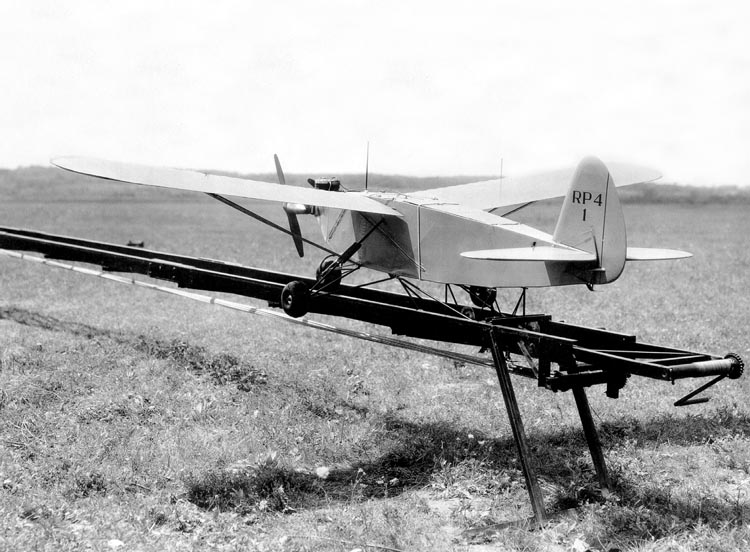
\includegraphics[width=0.8\textwidth]{/rp4.jpeg}}
\subfigure[Controlador de vuelo]{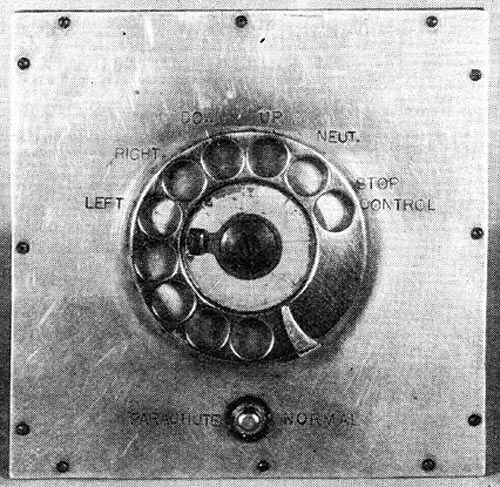
\includegraphics[width=0.6\textwidth]{/rp4controlador.jpeg}}
\caption[Caption]{RP-4 de Radioplane Company}
\label{fig:rp4}
\end{center}
\end{figure}

En la \textbf{Posguerra} de la \textbf{Segunda Guerra Mundial}, la compañía Radioplane produjo una serie de blancos aéreos no tripulados, llamados Falconer (ver Figura~\ref{fig:falconer}), que llevaban integrados sistemas de radiocontrol más modernos. 
Otra aplicación relevante durante la \textbf{Posguerra} fue la de señuelos antirradar. Estos eran soltados desde 
bombarderos, donde también eran controlados por radio con la ayuda de imágenes de vídeo, con la finalidad de confundir a los sistemas radar enemigos.

\begin{figure}[!h]
\begin{center}
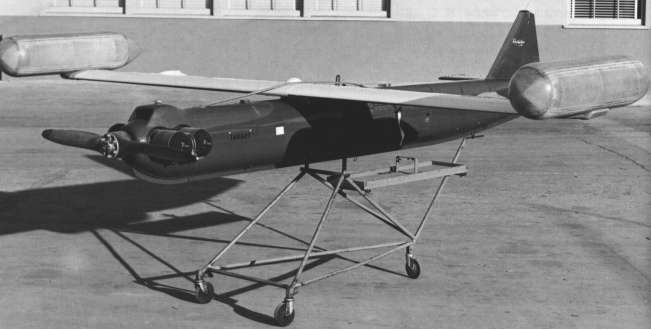
\includegraphics[width=0.8\textwidth]{/falconer.jpg}
\caption[Caption]{Northrop Falconer}
\label{fig:falconer}
\end{center}
\end{figure}

Con la aparición de aviones militares con sistemas de propulsión a reacción, a lo largo de \textbf{1960}
se desarrollaron blancos aéreos más rápidos y con mayor alcance. De esta manera, eran más difíciles de detectar y de derribar que los aviones de reconocimiento tripulados y, adicionalmente, no provocarían incidentes diplomáticos asociados con la captura de un piloto. 
Los \acs{UAV}s del momento fueron equipados con cámaras para misiones de reconocimiento, revelando las fotos en la base cuando el \acs{UAV} regresaba.
Algunos incluso incorporaron buscadores de radiación y cabezas de combate antirradar.

Los \textbf{años 70} iban a ser testigos de la inclusión de \acs{UAS} en misiones de 
reconocimiento y vigilancia tanto de corto alcance, como de largo alcance y elevada altitud. Fueron sistemas 
más complejos tanto en los requisitos de la misión como en la seguridad en las comunicaciones.

En \textbf{1890} se creó un sistema en el que el \acs{UAV} se lanzaba desde una rampa y se rescataba con un paracaídas y un airbag. 
Cuando se realizaban análisis diurnos el \acs{UAV} estaba equipado con una cámara convencional más una cámara de infrarrojos y para los análisis nocturnos únicamente se equipaba la cámara infrarroja. El guiado se llevaba a cabo mediante la preprogramación de un autopiloto basándose en giróscopos verticales y direccionales, información de altímetros y anemómetros barométricos. 
Además, transportaba un transmisor de video que podía enviar imágenes, en tiempo real, a la estación de control 
en tierra, estando a 70 km de la base.

En los \textbf{años 90} con la mayor disponibilidad del \acs{GPS} y de las comunicaciones vía satélite se consigue que los \acs{UAS} puedan operar por encima de la señal de radio y que puedan abandonar el uso de sistemas de navegación imprecisos basados en giróscopos y
datos de aire. Es así como, junto con los sistemas digitales de control de vuelo o \acs{DFCS}, el alcance y la precisión de la navegación mejoraron apreciablemente. 
Como resultado se desarrollaron sistemas de medio y largo alcance. 

En la \textbf{década de los 2000} se produce un incremento en el uso militar de los sistemas no tripulados. 
Por otro lado, las posibles aplicaciones civiles no han fructificado debido a la dificultad a la hora de asegurar la 
separación entre las aeronaves tripuladas y no tripuladas.
Otro paso adelante en esta década fue la instalación de armamento en \acs{UAV}s para una respuesta inmediata ante el posible 
descubrimiento de fuerzas enemigas.
Otras líneas de avance, en este periodo de tiempo, son las que tratan de aumentar la automatización, reduciendo así
la carga de trabajo y los errores de las tripulaciones en tierra.

\textbf{Más allá del 2010} el mercado militar de los \acs{RPAS} continúa con una tendencia positiva desde el final de la Guerra Fría y se espera que se acelere en las primeras décadas del siglo XXI.
La tendencia comercial en el mercado de la robótica está también en constante crecimiento, es por eso que la tecnología está apoyando estas tendencias, con microprocesadores cada vez más baratos y competentes que fomenten el desarrollo. 

\section{Cuadros}
\label{sec:uncuadro}

Se denominan «tablas» cuando contienen datos con relaciones numéricas. El
término genérico (que debe usarse cuando en los demás casos) es
«cuadro»~\cite{sousa}. Si las columnas están bien alineadas, las líneas
verticales estorban más que ayudan (no las pongas). Los cuadros se referencian
de este modo.


\section{Listados de código}
\label{sec:listado}

Puedes referenciar un listado así (ver Listado~\ref{code:hello}). Éste es un
listado flotante, pero también pueden ser «no flotantes» quitando el parámetro
\texttt{float} (mira el fuente de este documento o la referencia del paquete
\href{http://www.ctan.org/get/macros/latex/contrib/listings/listings.pdf}{«listings»}).

\begin{listing}[
  float=ht,
  language = C,
  caption  = {«Hola mundo» en C},
  label    = code:hello]
#include <stdio.h>
int main(int argc, char *argv[]) {
    puts("Hola mundo\n");
}
\end{listing}

\noindent
Puedes incluir un fichero de código fuente (o un fragmento) con \texttt{lstinputlisting}:

\lstinputlisting[language=C, firstline=3, texcl]{code/hello.c}

\noindent
Y también existe un comando \texttt{console} para representar ejecución de
comandos:

\begin{console}
$ uname --operating-system
GNU/Linux
\end{console} %$

Puedes modificar el estilo por defecto para tus listados añadiendo un comando
\texcmd{lstset} en tu \texttt{custom.sty}. El código \LaTeX{} del listado
\ref{code:custom-listings} añade un fondo gris claro y una línea en el margen
izquierdo.

\begin{listing}[
  float=h!,
  caption  = {Personalizando los listados de código},
  label    = code:custom-listings]
\lstset{%
  backgroundcolor = \color{gray95},
  rulesepcolor    = \color{black},
}
\end{listing}

En cualquier caso, si lo necesitas siempre es mejor que redefinas los comandos y entornos
existentes o crees entornos nuevos, en lugar de añadir los mismos cambios en
muchas partes del documento.



\section{Citas y referencias cruzadas}

Puedes ver aquí una cita~\cite{design_patterns} y una referencia a la segunda sección
(véase \S\,\ref{sec:uncuadro}). Para hacer referencias debes definir etiquetas en el punto
que quieras referenciar (normalmente justo debajo). Es útil que los nombres de las
etiquetas (comando label) tengan los siguientes prefijos (incluyendo los dos puntos ``:''
del final):

\begin{description}
\item[chap:] para los capítulos. Ej: ``\texttt{chap:objetivos}''.
\item[sec:] para secciones, subsecciones, etc.
\item[fig:] para las figuras.
\item[tab:] para las tablas.
\item[code:] para los listados de código.
\end{description}

Si estás viendo la versión PDF de este documento puedes pinchar la cita o el número de
sección. Son hiper-enlaces que llevan al elemento correspondiente. Todos los elementos que
hacen referencia a otra cosa (figuras, tablas, listados, secciones, capítulos, citas,
páginas web, etc.) son «pinchables» gracias al paquete
\href{http://latex.tugraz.at/_media/docs/hyperref.pdf}{\emph{hyperref}}.

Para citar páginas web usa el comando \texttt{url} como en: \url{http://www.uclm.es}


\section{Páginas}
\label{sec:paginas}

La normativa aconseja imprimir el documento a doble cara, pero si el número de
páginas es bajo puede imprimirse a una cara. Como eso es bastante subjetivo, mi
consejo es que ronde las 100 \textbf{hojas}. Una hoja impresa a doble cara
contiene 2 páginas, a una cara contiene una. Es decir, si el documento tiene más
de 200 páginas imprímelo a doble cara, si tiene menos imprímelo a una.

Por defecto, \esitfg{} imprime a una cara (oneside), si quieres imprimir a doble cara,
escribe en el preámbulo:

\begin{listing}
  \documentclass[twoside]{esi-tfg}
\end{listing}

Esto es importante porque a doble cara los márgenes son simétricos y a una cara
no. Si llevas el TFG a la copistería y pides que te lo impriman de modo
diferente al generado, quedará mal ¡Cuidado!

Tal como indica la normativa, los capítulos siempre empiezan en la página
derecha, la impar cuando se usa doble cara.


% Local Variables:
%  coding: utf-8
%  mode: latex
%  mode: flyspell
%  ispell-local-dictionary: "castellano8"
% End:
